\documentclass[a4paper,11pt]{article}

\usepackage[top=2.5cm, bottom=2.5cm, left=2.5cm, right=2.5cm]{geometry}

\usepackage{fancyhdr}
\pagestyle{fancy}
\fancyhf{}
\rhead{\thepage}

\usepackage{hyperref}

\usepackage{pdflscape}

\usepackage{graphics}
\usepackage{graphicx}

\usepackage{times}

% add paragraph breaks
\setlength{\parskip}{0.5em}
\renewcommand{\baselinestretch}{1.0}
\setlength{\parindent}{0em}

\title{Side Channel Attacks in the Browser}
\date{}
 
\begin{document}

\maketitle

\section*{Case for Support}

%a six-page (maximum) Case for Support: an account of the motivation for the work, the approach being taken, and a breakdown of the work to be carried out (often in terms of "workpackages"), plus a management plan (how will the project be managed such that it delivers what you have promised to do) and any other information that usefully describes the nature of the project being proposed)

\subsection*{Background}
Side-Channel Attacks (SCA) are an important class of cryptanalytic techniques which target unintentional information leakage in order to disclose private data. In general, Side-Channel attacks monitor a device performing an interesting operation and try to find a correlation between the side-channel information and the internal state of the processing device, which is related to the secret parameters involved in the computation. Side-channel information can be obtained by monitoring variations in the execution time (\textit{Timing Attacks}), the power consumption (\textit{Power Analysis}), the electro-magnetic emission (\textit{Electro-magnetic Analysis - EMA}), or the state of the cache memory (\textit{Cache Attacks}) \cite{standaert2010introduction}. The goal of an attacker in side-channel attacks is to either recover the secret parameters involved in the computation by targeting faults in the implementation of some cryptographic algorithm, or disclose private information about a user, such as their location or browsing history. Side-channel attacks exploit vulnerabilities in a specific implementation rather than targeting an abstract algorithm, making them less generic but more powerful \cite{standaert2010introduction}.

The expansion of the Internet determined browser vendors to add more and more features to their software in order to offer richer, dynamic and more interactive web pages. The evolution of browser software not only improved the overall user experience but also opened the way for a new category of side-channel attacks known as browser attacks. These types of attacks target vulnerabilities in the browser software. Browser attack fall into two categories: traditional timing attacks, which measure the time it takes the server to respond, and cache timing attacks, which use the time it takes to retrieve a resource in order to determine its origin, either local storage like the browser's cache memory, or a remote server.

Browser attacks are a very powerful category of side-channel attacks, which require minimal set up and affect a wide range of users. A basic browser attack requires a user to navigate to an untrusted website, which contains attacker-controlled content. The web page has a background script which collects information about the victim that can be used by the attacker to infer a user's location, browsing history, or even current browsing activity. The victims are usually unaware that the website is collecting private data about them. One might think that such attacks can be avoided by simply not visiting untrusted websites; however, researchers discovered that even high-profile websites are using similar techniques to collect information about their visitors\cite{jang2010empirical}. For example, a health insurance provider might want to know if the user has any health problems. If the user visited any health related web pages, they must be stored in the browser's cache memory, therefore an attacker who can investigate the state of the cache memory can find out what health issues the victim might have.

Compared to classic Side-Channel attacks, browser attacks appear and disappear at a faster rate. The majority of vulnerabilities found in the browser software get patched in less than a year. This gives attackers a limited time frame in which they can exploit potential vulnerabilities in web browsers. Sometimes the proposed countermeasure for certain browser attacks can severely impact the browser's performance and browser vendors choose not to include the fixes until a better solution is found. There is no guarantee that a countermeasure which does not impact the performance of the browser software will ever be found. There are browser attack discovered over fifteen years ago that have been improved over the years and are still in use today.

One of the first browser attack was discovered by Felten and Schneider\cite{felten2000timing} in 2000. Their attack measures the time it takes to retrieve a static web page and determines if it has been fetched from the browser's cache memory or from a remote server. An adversary can use this attack to disclose a user's browsing history. A few years later, Bortz et al.\cite{bortz2007exposing} identified a vulnerability in HTML, which allowed them to estimate the size of a remote file. Their work was extended by Van Goethem et al.\cite{van2015clock}, who used newer web development technologies in order to determine the size of a cross-origin resource.
 
Browser attacks are not only used to determine how much information a user has access to, in 2015 Jia et al.\cite{jia2015know} demonstrated that it is possible to determine a user's location. Additionally, Oren et al.\cite{oren2015spy} showed that it is possible to disclose a user's current browsing activity by analysing the state of their browser's cache memory.

\subsection*{Motivation}

The aforementioned papers present various techniques for disclosing private information about users, by either measuring the amount of data the users have access to, or simply determining what pages they previously accessed by checking the state of their browser's cache memory. Additionally, most of the papers present real world scenarios where the attacks can be used to de-anonymize a user; however, the attacks are presented from the perspective of a malicious user who is trying to gain access to private data. Our research is going to explore how browser attacks can be used by governmental organisations to obtain crucial information about a specific user.

In an attempt to offer more interactive, dynamic and richer web pages, in order to improve the overall user experience, browser vendors have been adding support for more and more features. Due to the rapid evolution of browser software, vulnerabilities are discovered and fixed within weeks. In general, adversaries have a limited time frame in which they can exploit potential browser vulnerabilities. Sometimes, adding a fix for a browser attack can severely impact the performance of the browser, hence, browser vendors avoid adding the countermeasure. Therefore, some browser attacks can be exploited for years until a better solution is found. This is the case of the attacks discovered by Felten et al.\cite{felten2000timing} and Bortz et al.\cite{bortz2007exposing}.

This motivated us to investigate new applications for this particular kind of browser attacks. Our research will target social network platforms and explore how side-channel information can be used to obtain a user's list of connections on social networking websites. In their paper, Van Goethem et al.\cite{van2015clock}, briefly mention a real world application of the browser attack in which they can determine if two people are friends on Facebook, or connected on LinkedIn. We are going to use their idea and efficiently determine a user's full list of contacts on any social network platform.

\subsection*{Project Objectives}

The aim of this research is to provide theory, tools and techniques for disclosing a user's list of connections on social media platforms. More specifically, we will focus on the following objectives:
\begin{enumerate}
\item To analyse known browser attacks which can be used to obtain hidden information from social media websites.
\item To build a web application which disclosed information about social network users.
\item To find new vulnerabilities in the browser software, which provide more efficient ways of estimating the size of a remote file.
\item To build a basic model which determines a user's connections on a small size internal social network website.
\item To use data provided by the Defence Science and Technology Laboratory (DSTL) in order to refine the algorithm.
\item To build a web application which discloses the full list of friends of a real world social network website user.
\item To run workshops for DSTL employees in order to increase awareness about browser attacks.
\end{enumerate}

\subsection*{Programme and Methodology}

Throughout this section we will refer to the list of a user's friends or connections on social media platforms as the \textbf{friend graph}.

\subsubsection*{Workpackage 1 (WP1) : A preliminary analysis of published attack vectors}
Research leader: Dr. Ana Dumitras, University of Bristol

Principle research objective:
\begin{quote}
	To review the existing literature on side-channel attacks in the browser and determine the efficiency of the attack vectors. Then we will implement a set of chosen browser attack which will later be used to determine the friend graph. Additionally, we will discover new vulnerabilities in the browser software which will provide more efficient results for estimating the size of a remote file.
\end{quote}

Principle deliverables:
\begin{enumerate}
\item Review existing literature on the most important side-channel attacks in the browser.
\item Provide implementations for the selected browser attacks, optimised to work on the most recent versions of browser software. 
\item Provide new attack vectors for estimating the size of a cross-origin resource.
\end{enumerate}

The goal of this package is to review existing attack vectors and analyse their efficiency in state-of-the-art browser software. Initially, this work package will focus on selecting a series of side-channel attacks in the web browser to be reviewed. We will use Semantics Scholar \cite{semanticsearch} and Google Scholar\cite{googlescholar} to identify the set of papers to be reviewed. In order to determine the friend graph in later WP3 and WP4 we need to select a specific set of side-channel attacks in web browsers. The criteria for selecting the papers is that they can be applied to real world scenarios where we are trying to determine the size of a remote file. Such attacks have been around for years and there are lots of resources available. 

The second task in this work package is to implement some of the selected browser attacks. Before implementing the attacks, we are going to theoretically determine if the attacks are still feasible. Even if the attacks are still possible, changes in the browser software will require additional work in order to run them on current versions of the browser software. The outcome of this work package is a series of browser attacks which work in the most popular browsers, such as Chrome, Firefox, Safari and IE. 

The third task, which is to be completed in parallel with WP1.2 implies finding new vulnerabilities in the browser software. We are going to use the information gained from reviewing past browser attacks and find similar patterns in new web development technologies. 

This work package is to be completed by a PhD student together with a PDRA, under the supervision of the Principal Investigator. The researchers are going to be supported by the Co-Investigator, who has experience in web development. The attack vectors which will be reviewed are to be determined by the researchers.

% WP2 web application for social media, being able to determine facts about a user
\subsubsection*{Workpackage 2 (WP2) : Build a model for answering yes-no questions about the user.}
Research leader: Dr. Ana Dumitras, University of Bristol

%rephrase
Principle research objective:
\begin{quote}
	To build a web applications which is able to answer yes or no questions about the victim's profile on social network websites.
\end{quote}

Principle deliverables:
\begin{enumerate}
\item Provide a web application which can be used to determine information about the victim.
\item A collection of tests for analysing the performance of the web application.
\end{enumerate}

This work package builds on the work from WP1, where we determine a set of suitable methods for estimating the size of a remote file. The goal of this work package is to build a web application which is able to infer certain information about a social media website user, such as group membership or if they have access to specific resources on the social media platform. More specifically, given a link to a resource on the social media website, our web application should be able to tell if the user has access to that resource or not by using techniques from WP1. This is similar to asking the application a series of questions whose answer's can only be yes or no.

The work is to be carried by a PhD student, under the supervision of the co-Investigator, who has experience in web applications and social media platforms. The criteria for success will be how  our web application guesses is certain facts about the user are true or false. Additionally, the application should be able to check if two users are connected, this would later be used in WP3. 

For ethical reasons we are not going to use data from actual users, but we are going to set up several accounts on the most popular social networks, like Facebook, Twitter or LinkedIn, and test our application on those accounts. These accounts will also be used for testing since we already know what answers to expect from the application.

\subsubsection*{Workpackage 3 (WP3) : Build model for determining the friend graph}
Research leader: Dr. Brian May, University of Bristol

%rephrase
Principle research objective:
\begin{quote}
	To extend the application developed in WP2 such that it works on a small size social network website provided by the Defence Science and Technology Laboratory (DSTL).
\end{quote}

Principle deliverables:
\begin{enumerate}
\item Provide a web application which discloses the friend graph on a small size social network.
\item A series of workshops to increase the awareness browser attacks.
\end{enumerate}

This work package focuses on disclosing the friend graph in a small size social network platform. As mentioned in WP2, for ethical reasons we are should not test out web application on real world social media platforms, like Facebook or LinkedIn, so the Defence Science and Technology Laboratory (DSTL) has agreed to provide us access to a internal social media platform where we are going to test our web application. 

In general, DSTL prefers work to be conducted by external suppliers. They are interested in being able to disclose the friend graph of social media users and have agreed to support our research by providing us with the needed data for developing the web application. DSTL is interested in learning more about vulnerabilities in social media platform and how to defend against them. As part if this work package we are going to organize workshops where DSTL's employees are going to learn more about browser attack and how they can be used to de-anonymize a user. 

The main goal of this work package is to have a web application which automatically displays the friend graph when given a link to a user's profile on DSTL's social network platform. The work is to be completed by a PhD student together with the PDRA, supervised by the PI. Additionally, DSTL is going to offer support by providing us with access to the internal social media platform. The success of this work package is measured in how accurately we can determine the friend graph on the given social network.

As part of this work package we are going to run a series of workshops to increase  awareness about browser attacks. The PDRA will be in charge of the workshops, additional support will be provided by the PI and CI.

\subsubsection*{Workpackage 4 (WP4) : Test the model on real world social networks}
Research leader: Dr. Brian May, University of Bristol

%rephrase
Principle research objective:
\begin{quote}
	To build a web application which discloses the friend graph of a user on a real world social media website.
\end{quote}

Principle deliverables:
\begin{enumerate}
\item Provide a web application for obtaining the friend graph of a user on a real world social media website.
\end{enumerate}

After the successful completion of WP3, we are going to focus on extending the web application to work on any social media platform. DSTL are interested in using our web application. The aim of this work package is to disclose the friend graph of a user of any social media website. This is going to be part of an ongoing project by DSTL which focuses on de-anonymising social network users who might pose a threat to national security.

The work will be completed by a PDRA, supervised by the PI. Since DSTL will be the main user of this application, they will provide additional support such as offering testing data and they will provide feedback during the implementation stage. Due to ethical reasons we are not allowed to test the application on random users. Dr. Roger Taylor from the Department of Law at the University of Bristol, who is specialized in Data Protection, is going to support our work during the development of this work package and provide any resources information needed for working with user data.

\subsection*{National Importance}

Our work is going to help the Defence Science and Technology Laboratory (DSTL), which are interested in discovering new applications for side-channel attacks in web browsers. Through our work with DSTL, we are contributing to the defence and security of the UK. Additionally, we will run several workshops aimed at increasing awareness about browser attacks, which should significantly decrease the number of users falling victims to browser attacks.

\subsection*{Academic Importance}


\bibliographystyle{unsrt}
\bibliography{research}

\newpage
\section*{Budget}

a one-page (maximum) Budget: a table/spreadsheet of expenditure


\begin{center}
\begin{tabular}{|l|l|}
\hline
Item & Cost for 3.5 years (\textsterling) \\\hline
PI & 140,000 \\\hline
CI1 & 70,000 \\\hline
CI2 & 70,000 \\\hline
PDRA & 350,000 \\\hline
PhD student & 100,000 \\\hline
Equipment & 10,240 \\\hline
International travel costs & 52,742 \\\hline
National travel costs & 15,366 \\\hline
Workshops & 5,346 \\\hline
\textbf{Total cost} & 813,694 \\\hline
\end{tabular}
\end{center}

\newpage
\section*{Justification For Resources}

%a one-page (maximum) Justification For Resources: essentially a written narrative on why you need the expenditure on each line-item in your budget

\subsection*{Directly incurred costs: staff}
There are five members from the University of Bristol involved in this research project. The Principal-Investigator will spend will spend 20\% of their time working on this project. Additionally, we will need two Co-Investigators, each will contribute 10\% of their time. The first CI will have a background in web development, while the second CI has experience in Data Protection and is going to provide support during the development of WP2, WP3 and WP4. The main research cost is the time of the PDRA and the PhD student.

\subsection*{Directly incurred costs: consumables}
\textsterling 4,000 is requested for PCs for the PDRA and the PhD student.

\textsterling 4,740 will be used to acquire additional equipment needed for implementing and testing platform specific attacks, such as mobile phones and tablets.

\textsterling 1,500 is going to be used to acquire any software licenses needed.

\subsection*{Directly incurred costs: travel and subsistence}
Budget has been allocated for each member to travel to several relevant conferences, such as COSADE: Constructive Side-Channel Analysis and Secure Design.

Additionally, \textsterling 15,366 are going to be used for travelling in order to collaborate with other academics or members from the industry.

\subsection*{Directly incurred costs: workshops}
We will run 5 workshops over the 3.5 years. \textsterling 5,346 is allocated to cover catering costs and any additional equipment needed for the workshops.
 

\newpage
\section*{Impact Statement}

%a one-page (maximum) Impact Statement: a description of how you intend to ensure that your work makes a difference in the world, rather than sitting on a shelf gathering dust)

The research proposal can be split into two parts: the first one which focuses on academic development by improving existing attacks, and a second part which aims to provide tools for the industry. The first part consists of WP1 and WP2, while the seconds part contains WP3 and WP4. 



\newpage
\begin{landscape}
\section*{Workplan}
%and also a one-page (maximum) Workplan:typically a GANTT chart or similar diagram indicating the order in which workpackages are carried out)

\begin{figure}[h]
\centering
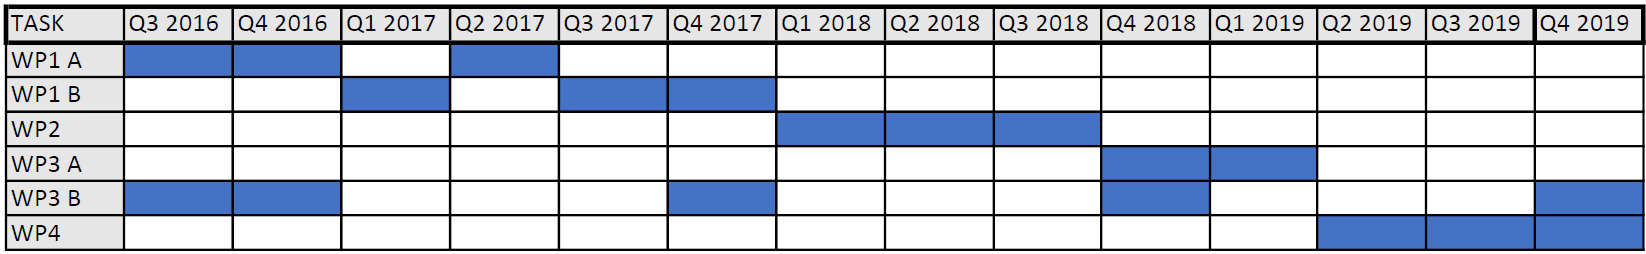
\includegraphics[width=25cm]{gantt.png}
\end{figure}

\subsection*{}

We are going to start with WP1 A, which requires an analysis of published attack vectors. After gathering enough data we can start work on WP1 B and for some time we are going to alternate the two tasks. By the end of WP1 we are going to focus entirely on the implementation part described in WP B. After completing WP1 we can start working on WP2. Once WP2 is completed, DSTL is going to provide the data needed for WP3 A and with the resources obtained from WP2 we can start working on the current work package. The outcome from WP3 A is going to be used in WP4. WP3 B is going to start at the same time as WP1. We are going to have two workshops in the first two quarters, and then one workshop during the last quarter of the next three years.

\end{landscape}
\end{document}